\documentclass[a4paper]{article}

%% Language and font encodings
%\usepackage[english]{babel}
\usepackage[spanish]{babel}
\usepackage[utf8x]{inputenc}
\usepackage[T1]{fontenc}

%% Sets page size and margins
\usepackage[a4paper,top=3cm,bottom=2cm,left=3cm,right=3cm,marginparwidth=1.75cm]{geometry}

%% Useful packages
\usepackage{amsmath}
\usepackage{graphicx}
\usepackage[colorinlistoftodos]{todonotes}
\usepackage[colorlinks=true, allcolors=blue]{hyperref}

\title{Procesamiento digital de señales de audio - Hoja 1}
\author{Julieta Umpierrez}
\date{\vspace{-5ex}}
\begin{document}
\maketitle

\section{Ejercicio 1 }

Digitalización. Sampling, aliasing. Cuantización. Dithering.
Este ejercicio tiene como objetivo estudiar el muestreo y la cuantización de señales de audio.

\subsection{Parte 1- Sampling y aliasing}
Por el teorema de muestreo se tiene que si $f_s$ es la frecuencia de muestreo y $f_{max}$ es la frecuencia máxima de la señal, estas deben cumplir que $f_s>2f_{max}$ para que no exista aliasing. 
\newline
En el caso del audio tones.wav se tienen dos tonos, uno de 1760Hz para el cual la $f_s$ debe cumplir que $f_s>3520Hz$ y un segundo tono de 7040Hz para el cual la $f_s$ debe cumplir que $f_s>14080Hz$. Es por eso que teóricamente se espera que al remuestrear a $fs = \frac{44100}{2}Hz = 22050Hz $ y a $fs = \frac{44100}{4}Hz = 11025Hz$ el primer tono se comporte igual y el segundo tono cambie en la ultima frecuencia de muestreo pues se deja de cumplir la condición para que no exista aliasing.

\newline 
Para estudiar esto se remuestreo cambiando la frecuencia de muestreo y tomando cada dos y cuatro muestras respectivamente y se realizaron los espectrogramas correspondientes. Con esto se pudo constatar la correspondencia con lo esperado teóricamente ya que en el caso de $f_s = 11025Hz $ el segundo tono se escucho de manera diferente, mas formalmente esto se puede evidenciar en la figura \ref{comparacion1} donde la gráfica de la izquierda muestra el espectrograma de la señal original con las bandas de frecuencia cercanas a $1760Hz$ y $7040Hz$ mientras que en la figura de la derecha se ve claramente el efecto del aliasing al cambiar la banda de $7040Hz $ a algo cercano a $4000Hz$.

\begin{figure}[h]
\begin{minipage}[b]{0.5\linewidth}
\centering
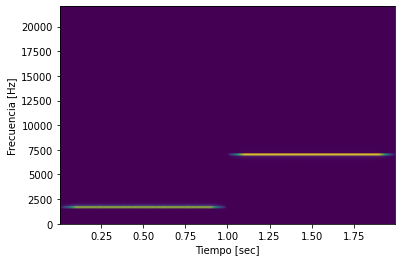
\includegraphics[width=\linewidth]{original_tones.png}
\caption{Espectrograma de señal original}
\label{f:figura1}
\end{minipage}
\hspace{0.5cm}
\begin{minipage}[b]{0.5\linewidth}
\centering
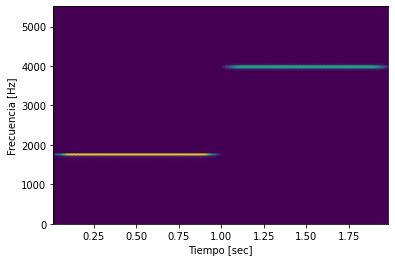
\includegraphics[width=\linewidth]{4_tones.png}
\caption{Espectrograma $f_s = 11025Hz$}
\label{f:figura2}
\end{minipage}
\caption{Comparación de espectrogramas con el primer método.}
\label{comparacion1}
\end{figure}
\newline
Luego se repitió este análisis pero con otro método, utilizando la función decimate de scipy signal. Esta función realiza el remuestreo luego de aplicar un filtro antialias por lo que para el segundo tono, a $f_s = 11025Hz$ no se escucha nada ni se ve nada en el espectrograma como se muestra en la figura \ref{comparacion2}.
\begin{figure}[h]
\begin{minipage}[b]{0.5\linewidth}
\centering
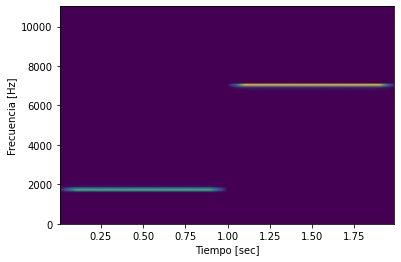
\includegraphics[width=\linewidth]{2_tonesd.png}
\caption{Espectrograma a $f_s = 22050Hz$}
\label{f:figura1}
\end{minipage}
\hspace{0.5cm}
\begin{minipage}[b]{0.5\linewidth}
\centering
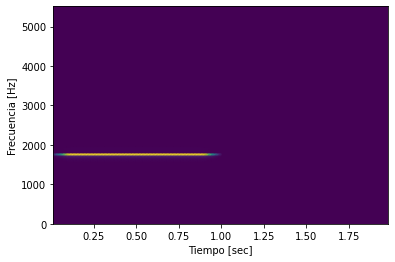
\includegraphics[width=\linewidth]{4_tonesd.png}
\caption{Espectrograma $f_s = 11025Hz$}
\label{f:figura2}
\end{minipage}
\caption{Comparación de espectrogramas con el segundo método.}
\label{comparacion2}
\end{figure}


\newline
Para el audio chirp.wav primero se realizo un análisis con Audacity en el cual se evidencio que era una señal compuesta por tonos de distintas frecuencias que iban en aumento. Esto se puede ver claramente en la figura \ref{chirp}. En este caso ya en la primer frecuencia de muestreo nueva, es decir $f_s = 22050Hz$ ya se escuchan cambios a partir de los 5s que en la gráfica \ref{chirp} se correspondía con aproximadamente $11000Hz$ que es cercano al limite de aliasing impuesto por el teorema de muestreo.
En el caso de $f_s = 11025Hz$ los cambios se escuchan a partir de los 3s que en la gráfica \ref{chirp} se correspondía con aproximadamente $5500Hz$  que es cercano al limite de aliasing como en el caso anterior. 

\begin{figure}[h]
\centering
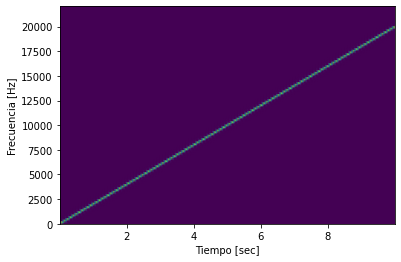
\includegraphics[width=0.5\textwidth]{chirps.png}
\caption{Espectrograma de audio chirp.wav a $f_s = 44100z$}
\label{chirp}
\end{figure}

\newline 
Con el segundo método, sucede lo mismo que en el caso anterior, cuando eligiendo cada 2 o 4 muestras cambiaba el audio, en este caso desaparece. Esto se evidencia en la comparación de espectrogramas de la figura \ref{comparacion3}, en la cual se ve claramente el efecto del filtro antialias. 
\begin{figure}[h]
\begin{minipage}[b]{0.5\linewidth}
\centering
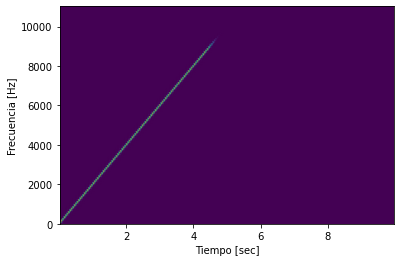
\includegraphics[width=\linewidth]{caso1.png}
\caption{Espectrograma $f_s = 22050Hz$ }
\label{f:figura1}
\end{minipage}
\hspace{0.5cm}
\begin{minipage}[b]{0.5\linewidth}
\centering
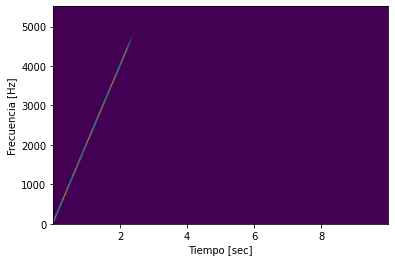
\includegraphics[width=\linewidth]{caso2.png}
\caption{Espectrograma $f_s = 11025Hz$}
\label{f:figura2}
\end{minipage}
\caption{Comparación de espectrogramas con el segundo método.}
\label{comparacion3}
\end{figure}



\subsection{Parte 2- Quantization / Dithering}
Asumiendo un error de cuantización uniforme con distribución $U(-Q/2,Q/2)$ y que la entrada es una señal de amplitud máxima $Xpeak$ se puede calcular el Signal to Error Ratio (SER) como:
$$
SER = \bigg[\frac{Srms}{Erms}\bigg]^2
$$
donde $Srms$ es el valor rms de la señal de entrada y $Erms$ es el error de cuantización rms. 

\newline
Dado que el intervalo de cuantización es $Q$, si se considera una palabra de $n$ bits, hay $2^n$ intervalos de cuantización por lo que
$$
Q = \frac{2Xpeak}{2^n} \Rightarrow Xpeak = Q2^{(n-1)} 
\Rightarrow Srms = \frac{Q2^{(n-1)}}{\sqrt{2}}
$$

\newline
Por definición se tiene que $Erms = \bigg[\int^{-\infty}_{-\infty} e^2p(e)de\bigg]^{1/2}$. Utilizando la distribución de probabilidad del error y resolviendo la integral se tiene que:
$$
Erms = \bigg[\frac{1}{Q}\int_{-Q/2}^{Q/2} e^2de\bigg]^{1/2}
= \bigg[\frac{1}{Q}\frac{e^3}{3}\bigg|^{Q/2}_{-Q/2}\bigg]^{1/2}
= \bigg[\frac{1}{3Q}\bigg(\frac{Q^3}{8}+\frac{Q^3}{8}\bigg)\bigg]^{1/2}
= \bigg[\frac{Q^2}{12}\bigg]^{1/2}
= \frac{Q}{\sqrt{12}}
$$

\newline
Ahora se puede calcular la $SER$ utilizando la definición y realizando algunas cuentas
$$
SER = \bigg[\frac{Q2^{n-1}}{\sqrt{2}}\frac{\sqrt{12}}{q}\bigg]^2
= \bigg[\frac{2^n}{2\sqrt{2}}\sqrt{12}\bigg]^2 
= \frac{3}{2}2^{2n}
$$

\newline
Utilizando que $(SER)db = 10log(SER)$ se tiene que
$$
(SER)db = 10log(3/2) + 10log(s^{2n}) = 10log(3/2) +20log(2)n \approx 1.761 + 6.021n
$$
esta ultima expresión muestra que cada bit que se agrega a la palabra aumenta el Signal to Error Ratio en 6db o lo que es equivalente, genera una disminución de 6db en el error de cuantización.

\newline
El dither consiste en agregar ruido no colacionado con la señal de audio para que el error de cuantización se decorrelacione de la señal. Por lo que la potencia del ruido total va a ser la suma entre la potencia del ruido de cuantización sin dither y la del dither. La potencia se calcula como se calculo $Erms$ pero sin la raiz pues no se quiere obtener el valor $rms$, esto es lo mismo que calcular $\sigma^2$ o varianza de la distribución. Esto implica que la potencia del error de cuantización sin dither es $\frac{Q^2}{12}$

\newline
En el caso de la pdf triangular 
$$
Pot_{triang} = \int_{-Q}^{0}e^2\bigg[\frac{e}{Q^2}+\frac{1}{Q}\bigg]de + \int_{0}^{Q}e^2\bigg[\frac{-e}{Q^2}+\frac{1}{Q}\bigg]de
= \bigg[\frac{e^4}{4Q^2} + \frac{e^3}{3Q}\bigg]\bigg|_{-Q}^{0}
+ \bigg[\frac{-e^4}{4Q^2} + \frac{e^3}{3Q}\bigg]\bigg|_{0}^{Q}
= \frac{Q^2}{6}
$$
Por lo que 
$$
Pot_{tot triangular} = \frac{Q^2}{12} + \frac{Q^2}{6}
$$

\newline
En el caso de la pdf uniforme es la misma distribución que se había considerado para el ruido de cuantización por lo que 

$$
Pot_{tot rect} = \frac{Q^2}{12} + \frac{Q^2}{12}
$$

\newline
En el caso de la pdf gaussiana $\sigma^2 = \frac{Q^2}{4}$ por lo que 
$$
Pot_{tot gaussiano} = \frac{Q^2}{12} + \frac{Q^2}{4}
$$

\newline
A continuación se pusieron en practica estos resultados teóricos para una sinusoide de amplitud 2 y  frecuencia $500Hz$ muestreada a $f_s = 44100Hz$. Para eso se sumaron los tres tipos de dither y luego se cuantizaron todas las señales. En primer lugar al agregar los dithers se escucha la señal original sin cambios pero con un ruido arriba. Al cuantizar la señal original se obtiene el resultado presentado en la figura \ref{sinusoide_c} que al escucharse suena sin ruido pero con una diferencia grande en cuanto a lo que se escucha. 

\begin{figure}[h]
\centering
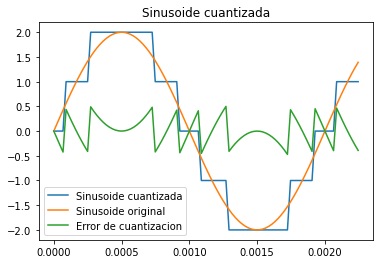
\includegraphics[width=0.5\textwidth]{sinusoide_c.png}
\caption{Sinusoide cuantizada}
\label{sinusoide_c}
\end{figure}

Cuando se cuantiza las señales con dither, sigue existiendo ruido pero se vuelve a escuchar el audio de manera muy similar a como se escuchaba previo a la cuantización. En la tabla \ref{tabla} se adjunta la comparación entre la potencia del ruido en cada caso de estudio. Claramente el del menor ruido es la cuantización sin dither y de los que tienen dither el de menor potencia es el de dither rectangular como era esperado. 

\begin{table}[]
\centering
\begin{tabular}{ll}
Dither & Potencia del ruido \\
Sin dither & 0.069 \\
Triangular & 0.21 \\
Rectangular & 0.14 \\
Gaussiano & 0.27
\end{tabular}
\label{tabla}
\caption{Comparación de la potencia del ruido en cada caso}
\end{table}

\newline
Además de la diferencia perceptiva entre la cuantización de la señal con y sin dither, esta se puede evidenciar con la comparación de espectros que se realiza en las figuras \ref{fftsin}, \ref{fftcon} y \ref{fftrect} en la cual se aprecia que a pesar del ruido es la señal cuantizada con dither la que tiene el espectro mas parecido a la original. 
\begin{figure}[h]
\centering
\begin{minipage}{0.45\textwidth}
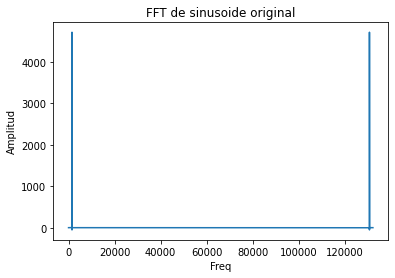
\includegraphics[width=\textwidth]{fftsinusoide.png}
\caption{Sin cuantizar}
\label{fftsin}
\end{minipage}\hfill
\begin{minipage}{0.45\textwidth}
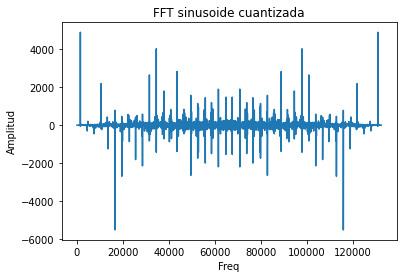
\includegraphics[width=\textwidth]{fftcuant.png}
\caption{Cuantizada}
\label{fftcon}
\end{minipage}\par
\vskip\floatsep% normal separation between figures
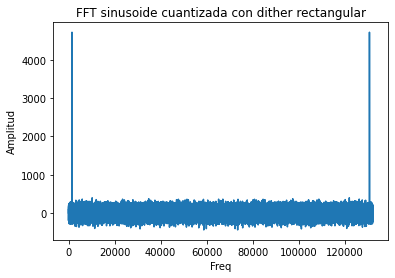
\includegraphics[width=0.45\textwidth]{fftrect.png}
\caption{Cuantizada con dither rectangular}
\label{fftrect}
\end{figure}
\newpage
\section{Ejercicio 2}
En este ejercicio se calculan características en tiempo corto de una señal de audio; en particular, energía, magnitud y tasa de cruces por cero.
\subsection{Parte 1}
En esta parte el objetivo es calcular expresiones para la energía y la magnitud de tiempo corto con diferentes ventanas. Para realizarlo se hará uso del diagrama presentado en la figura \ref{diagrama},
\begin{figure}[h]
\centering
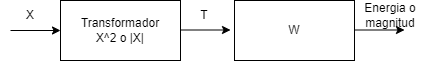
\includegraphics[width=0.5\textwidth]{drawio.png}
\caption{Diagrama de bloques para el calculo de la energía y magnitud de tiempo corto}
\label{diagrama}
\end{figure}
dada las definiciones para la energía y magnitud de tiempo corto se puede ver que son convoluciones de diferentes transformaciones de la entrada con la ventana, es por eso que se decidió trabajar en el dominio de la frecuencia para obtener ecuaciones recursivas que determinen el calculo. 

\newline
En el caso de 
		$$w_a[n]=
			\begin{cases}
				a^n, & n \geq 0 \\
				0, & n < 0.
		\end{cases}	$$
realizando la transformada Z se obtiene 
$$
W_a(z) = \frac{1}{1-az^{-1}} = \frac{Salida(z)}{T(z)}
$$
Antitransformando se tiene que 
$$
Salida[n] - aSalida[n-1] = T[n]
$$
En términos de los resultados buscados,
$$
E[n] = X^2[n] + aE[n-1]
$$
y 
$$
M[n] = |X[n]| +aM[n-1]
$$

\newline
Cuando la ventana es
$$
w_R[n]=
			\begin{cases}
				1, & 0 \leq n \leq N-1 \\
				0, & \text{en otro caso}.
			\end{cases}
$$
se tiene que $E_n  =  \sum_{m=-\infty}^{\infty}x^2[m]w[n-m]$ y
$ M_n  = \sum_{m=-\infty}^{\infty}|x[m]|w[n-m]$ y por los limites donde la ventana vale 1 se tiene que 
$$
E_n  =  \sum_{m=n-N+1}^{n}x^2[m]
$$
$$
M_n  =  \sum_{m=n-N+1}^{n}|x[m]|
$$
a partir de esto se pueden crear funciones que calculen estos valores de acuerdo a esta ventana, en este caso estas funciones se testearon utilizando el archivo $voice.wav$ que se adjunta graficado en la figura \ref{voicewav} donde se identifican momentos de gran amplitud donde se identificaría la voz y momentos de amplitud nula que serian las pausas.
\begin{figure}[h]
\centering
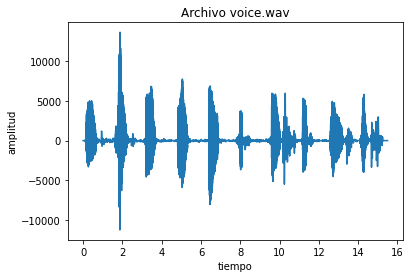
\includegraphics[width=0.5\textwidth]{voicewav.png}
\caption{Señal del archivo voice.wav}
\label{voicewav}
\end{figure}

\newline
En las figuras \ref{energia} y \ref{magnitud} se adjuntan las gráficas correspondientes a la energía y magnitud de tiempo corto de esta señal respectivamente, ambas se realizaron para una ventana de largo 640 pues dado que la $f_s = 16kHz$ se utilizo una ventana de $40ms$. 
\begin{figure}[h]
\begin{minipage}[b]{0.5\linewidth}
\centering
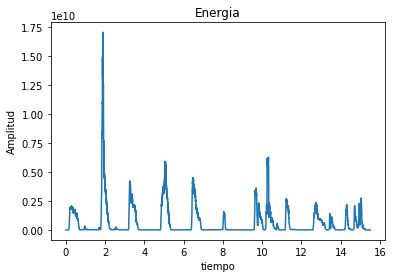
\includegraphics[width=\linewidth]{energia.png}
\caption{Energía de tiempo corto }
\label{energia}
\end{minipage}
\hspace{0.5cm}
\begin{minipage}[b]{0.5\linewidth}
\centering
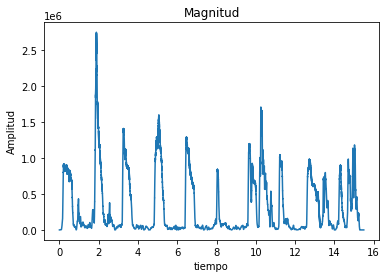
\includegraphics[width=\linewidth]{magnitud.png}
\caption{Magnitud de tiempo corto}
\label{magnitud}
\end{minipage}
\caption{Energía y magnitud de tiempo corto para el archivo $voice.wav$}
\label{eym}
\end{figure}
Si la SNR es alta, la energía permite la distinción entre sonido y silencio, lo que podría usarse para encontrar el comienzo y final de las palabras. Esto se ve claramente en el ejemplo y en contraposición con la magnitud de tiempo corto pues en las regiones donde debería haber silencio, es la energía de tiempo corto la que genera la función mas "suave".

\newline
\subsection{Parte 2}
Análogamente a como se definió la energía y la magnitud de tiempo corto para la ventana rectangular, se puede usar el mismo razonamiento de acuerdo a los limites donde vale $1/2N$ la ventana para tener esta forma mas compacta de la formula de tasa de cruces por cero

$$
Z_n = \frac{1}{2N}\sum_{m=n-N+1}^{n} |sign(x[m])-sign(x[m-1])|
$$

si se quiere escribir de forma recursiva utilizando $Z_{n-1}$  se debe tener en cuenta que 
$$
Z_{n-1} = \frac{1}{2N}\sum_{m=n-1-N+1}^{n-1} |sign(x[m])-sign(x[m-1])|
$$
esto implica que a $Z_n$ se lo corrió un lugar a la izquierda lo que genero que apareciera un nuevo termino y desapareciera otro. Es por eso que para escribirlo de manera recursiva hay que sumar el termino que falta que es en $m =  n$ y restarle el nuevo que es en $m = n-N$, estos términos son $|sign(x[n])-sign(x[n-1])|$ y $|sign(x[n-N])-sign(x[n-N-1])|$  respectivamente es por eso que la expresión recursiva queda

$$
Z_n = Z_{n-1} +\frac{1}{2N}\big[|sign(x[n])-sign(x[n-1])| - |sign(x[n-N])-sign(x[n-N-1])|\big]
$$

\newline
En la gráfica de la figura \ref{cero} se presenta la tasa de cruces por cero para el archivo $voice.wav$ utilizando una ventana de $10ms$ que corresponden a $N = 160$. Este calculo puede ayudar en la distinción de silencio y voz para aportar mas información acerca de los sonidos fricativos, esto se ve especialmente al rededor de los 8s donde la energía marca un pequeño pico que al escuchar el audio sabemos que corresponde a la palabra 'six' y añadiendo la información de la tasa de cruces por cero se ve que en ese momento no hay silencio como se podría haber pensado por la energía. 
\begin{figure}[h]
\centering
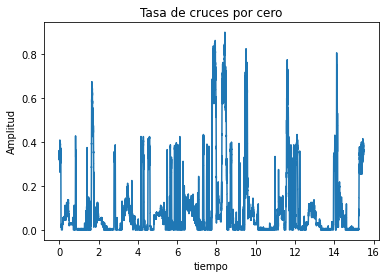
\includegraphics[width=0.5\textwidth]{cero.png}
\caption{Tasa de cruces por cero de voice.wav}
\label{cero}
\end{figure}

\newline
\subsection{Parte 3}
En esta parte se intentara realizar un algoritmo para el reconocimiento del inicio y final de palabras utilizando la energía de tiempo corto y la tasa de cruces por cero. Para eso, a través de las figuras \ref{energia} y \ref{cero} se estableció un umbral para cada magnitud a partir del cual se considera que hay voz y así ver el principio y el final de las palabras. En el algoritmo se calculan estas magnitudes y se ve muestra a muestra en primer lugar si la energía pasa el umbral, de ser así se detecta que hay voz, en el caso de que eso no suceda se chequea el umbral para la tasa de cruces por cero que busca detectar los sonidos fricativos como fue explicado anteriormente. Esto se aplico a tres archivos diferentes y los resultados se adjuntan en las figuras \ref{voice}, \ref{voice2} y \ref{fox}. En esas figuras se ve claramente que el enfoque para resolver el problema funciona relativamente bien en el primer audio, muy mal en el segundo y que tiene un mejor desempeño que en voice2.wav pero igual es muy malo. Esto se debe a varias razones, la primera es los umbrales que fueron los mismos para las tres señales cuando estos se habían elegido teniendo voice.wav en mente, por lo que se podría volver a realizar la evaluación de energía y tasa de cruces por cero para elegir umbrales mas adecuados en cada caso. En segundo lugar se podrían afinar las elecciones tomando en cuenta que la señal se mantenga por sobre un umbral durante un determinado intervalo para evitar ruidos o introduciendo otras magnitudes o diferentes anchos de ventana de acuerdo a como se comporta el audio. 
\begin{figure}[h]
\centering
\begin{minipage}{0.45\textwidth}
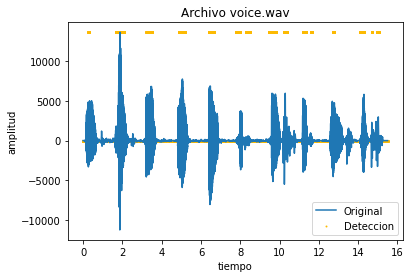
\includegraphics[width=\textwidth]{deteccion.png}
\caption{Archivo voice.wav}
\label{voice}
\end{minipage}\hfill
\begin{minipage}{0.45\textwidth}
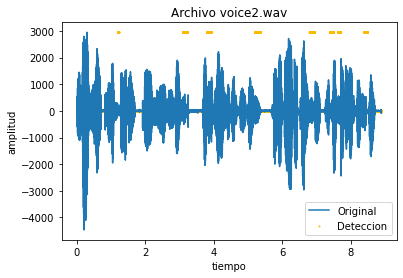
\includegraphics[width=\textwidth]{voice2.png}
\caption{Archivo voice2.wav}
\label{voice2}
\end{minipage}\par
\vskip\floatsep% normal separation between figures
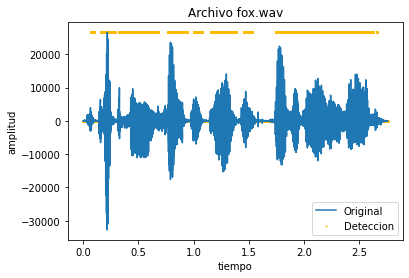
\includegraphics[width=0.45\textwidth]{fox.png}
\caption{Archivo fox.wav}
\label{fox}
\end{figure}






\section{Ejercicio 3}
En este ejercicio se presenta el cálculo de la función de autocorrelación, y su aplicación en el cálculo de la frecuencia fundamental de una señal de audio.
\subsection{Parte 1}
A continuación se demostrara que la autocorrelación es una función par pues 
$$
R_n[k] = \sum_{m=-\infty}^{\infty}x[m]w[n-m]x[m+k]w[n-k-m] \overbrace{=}^{\tau = m+k} 
\sum_{\tau=-\infty}^{\infty}x[\tau - k]w[n-\tau +k]x[\tau]w[n-\tau] $$
$$
= \sum_{\tau=-\infty}^{\infty} x[\tau]w[n-\tau]x[\tau-k]w[n-\tau+k]
= R_n[-k]
$$
donde el segundo renglón es reordenando e identificando la forma de la autocorrelación pero para $-k$.
A partir de que es par se puede escribir la autocorrelación de una manera mas compacta utilizando lo siguiente
$$
R_n[k] = R_n[-k] = \sum_{m=-\infty}^{\infty} x[m]w[n-m]x[m-k]w[n+k-m] = 
\sum_{m=-\infty}^{\infty} x[m]x[m-k]w[n-m]w[n-m+k] $$
$$= 
\sum_{m=-\infty}^{\infty} x[m]x[m-k]h_k[n-m]
$$
tomando $h_k[n] = w[n]w[n+k]$

\subsection{Parte 2}
En esta parte se utilizara la autocorrelación en tiempo corto con una ventana rectangular para la detección de la frecuencia fundamental de una señal de audio. Se utilizara la siguiente ventana
$$
w_R[n]=
			\begin{cases}
				1, & 0 \leq n \leq N-1 \\
				0, & \text{en otro caso}.
			\end{cases}
$$
por lo que la autocorrelacion es 
$$
R_n[k] = \sum_{m=n+k-N+1}^{n} x[m]x[m-k]
$$
La idea es entonces tomar 250 valores de autocorrelación por frame y buscar el primer índice donde esta autocorrelación supere el $60\%$ del valor en cero ya que eso implica un componente periódico en $f = \frac{f_s}{indice}$. A su vez, dado que la voz humana no tiene frecuencias fundamentales mayores a los $1000Hz$, se setean manualmente a 0 todas las frecuencias que hayan arrojado ese resultado. Los resultados de esto se adjuntan en la figura \ref{fund}. Lamentablemente este resultado no es parecido al obtenido a través del archivo txt, es por eso que es muy probable que haya errores en la implementación de este algoritmo. Al comparar con el resultado esperado se puede ver que uno de los problemas es que se esta detectando el índice que supera el $60\%$ antes de lo esperado lo que indicaría un error en el calculo de la autocorrelación. A su vez se intento con un enfoque vectorial para el calculo de la autocorrelación que también fallo dado que detecta los máximos mucho antes que la otra implementación. Los resultados se adjuntan en la figura \ref{fundpeor}. 
En resumen, no solo los resultados están mal por que no se parecen al resultado esperado si no que también están estimando frecuencias fundamentales que no se corresponden con las de la voz humana. 
Lo primero a mejorar seria encontrar el bug en la implementación, ya sea la versión con la sumatoria o la vectorial. Luego de arreglar eso se podría cambiar el valor del umbral de detección y ponerlo mas alto, es decir aumentar ese $60\%$ e incluso cambiar la forma de calcular la autocorrelación utilizando la autocorrelación modificada mencionada en clase encontrando el retardo de la segunda ventana que mejor se ajuste al problema. 

\begin{figure}[h]
\centering
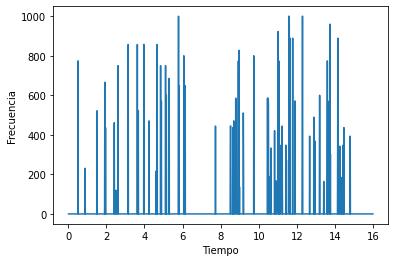
\includegraphics[width=0.5\textwidth]{fundamental.png}
\caption{Estimación de frecuencia fundamental}
\label{fund}
\end{figure}

\begin{figure}[h]
\centering
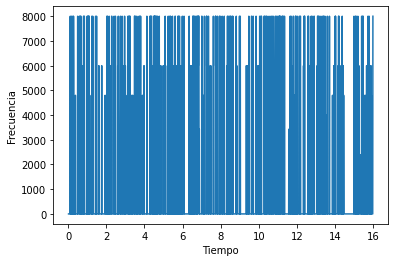
\includegraphics[width=0.5\textwidth]{mal.png}
\caption{Estimación de frecuencia fundamental}
\label{fundpeor}
\end{figure}

\newpage
\begin{thebibliography}{100} % 100 is a random guess of the total number of
%references
\addtolength{\leftmargin}{0.2in} % sets up alignment with the following line.
\setlength{\itemindent}{-0.2in}
\bibitem[Pohlmann]{Pohlmann11}Pohlmann, K. C. (Ed.). (2011). Fundamentals of digital audio. In Principles of Digital Audio (Sixth ed., pp. 28–44). McGraw-Hill Education.
\bibitem[Rabiner11]{RS} Rabiner, L. R., & Schafer, R. W. (2011). Time-domain methods for speech processing. In Theory and Applications of Digital Speech Processing (First ed., pp. 239–277). Pearson.
\bibitem[OF1]{of1} [Introducción al procesamiento de audio], [Martin Rocamora], Proyecto OpenFING, [https://open.fing.edu.uy/courses/audiodsp/1], publicado bajo una licencia CC By NC ND.
\bibitem[OF2]{of2}[Procesamiento en el dominio del tiempo], [Martin Rocamora], Proyecto OpenFING, [https://open.fing.edu.uy/courses/audiodsp/3], publicado bajo una licencia CC By NC ND.
\end{thebibliography}









\end{document}